\documentclass[12pt]{article}

\usepackage[margin=1in]{geometry}
\usepackage{listings,color,verbatim,graphicx,caption,url}
\definecolor{mygreen}{rgb}{0,0.6,0}
\definecolor{mygray}{rgb}{0.5,0.5,0.5}
\definecolor{mymauve}{rgb}{0.58,0,0.82}
\lstset{ %
  backgroundcolor=\color{white},   % choose the background color
  basicstyle=\scriptsize,        % size of fonts used for the code
  breaklines=true,                 % automatic line breaking only at whitespace
  captionpos=b,                    % sets the caption-position to bottom
  commentstyle=\color{mygreen},    % comment style
  escapeinside={\%*}{*)},          % if you want to add LaTeX within your code
  keywordstyle=\color{blue},       % keyword style
  stringstyle=\color{mymauve},     % string literal style
}

% section formatting
\usepackage{titlesec}
\titleformat*{\section}{\large\bfseries}
\titleformat*{\subsection}{\normalsize\bfseries}
\titlespacing\section{0pt}{12pt plus 4pt minus 2pt}{2pt plus 2pt minus 2pt}
\titlespacing\subsection{0pt}{12pt plus 4pt minus 2pt}{2pt plus 2pt minus 2pt}

\begin{document}
\noindent \textbf{\Large mdalayzer: A Molecular Dynamics Analysis Package}

\vspace{2mm}
\noindent \large November 21, 2014
\vspace{5 mm}

\noindent \large \textbf{Group Members:}
\vspace{1 mm}

\noindent \large Mike Howard (\url{mphoward@princeton.edu})
\vspace{1 mm}

\noindent \large Sang Beom Kim (\url{sangbk@princeton.edu})
\vspace{1 mm}

\noindent \large Andrew Santos  (\url{apsantos@princeton.edu})
\vspace{1 mm}

\noindent \large Elia Altabet  (\url{altabet@princeton.edu})
\vspace{1 mm}

\noindent \large Joey Vella (\url{vella@princeton.edu})

\section{Overview}
We will create a package that can be used to analyze trajectories from molecular dynamics simulations.  Molecular dynamics is a simulation method where Newton's equations of motions are solved for a set of particles in a given interatomic potential. Molecular dynamics has been extremely successful in simulating a wide range of materials and phenomena, and serves as a powerful complement to experimental studies. Various structural and thermodynamic properties of interest can be derived from the molecular trajectory both on the microscopic and macroscopic scale. These properties are usually calculated by post-processing simulation data.

Currently, a variety of well-developed packages exist for performing molecular dynamics simulation on multiple CPUs or GPUs, including GROMACS, LAMMPS, and HOOMD-blue. However, each of these simulation packages outputs trajectories in a variety of formats, including individual ASCII snapshot frames (.xyz, .xml, .gro, .pdb, etc.) and complete binary trajectories (.dcd, .xtc, .trr, etc.). Some simulations are conducted using in-house or legacy codes, which may output frames in customized or archaic tabular formats.

The vast array of available trajectory file formats considerably complicates writing code to perform post-simulation analysis. This often leads to duplication of coding efforts to perform simple tasks, or necessitates interconversion between file formats. Our software, mdalyzer, will vastly simplify this process through a highly extensible Python/C++ module that allows for reading of a variety of typical or customized trajectories that may be analyzed using a standard �toolbox�.

This toolbox will include methods to calculate the mean-square displacement, the velocity autocorrelation function, density and temperature profiles, the pair distribution function, and the static structure factor.  We will also be able to identify the presence of clusters. This toolbox can be easily extended by the user to include other compute methods through the C++ API.
	
We note that there currently exist some tools for reading and converting molecular dynamics trajectories.  However, typically analysis scripts still need to be written in these programs. Our software improves on these codes in three important ways: (1) less work is required for the user conducting �standard� calculations, (2) C++ computes may calculate on large trajectories faster than scripted computes, and (3) our software is easily extended in C++ for the user reading a new file format or performing a new compute.

\section{Architecture}
\begin{figure}[!htbp]
 \centering
 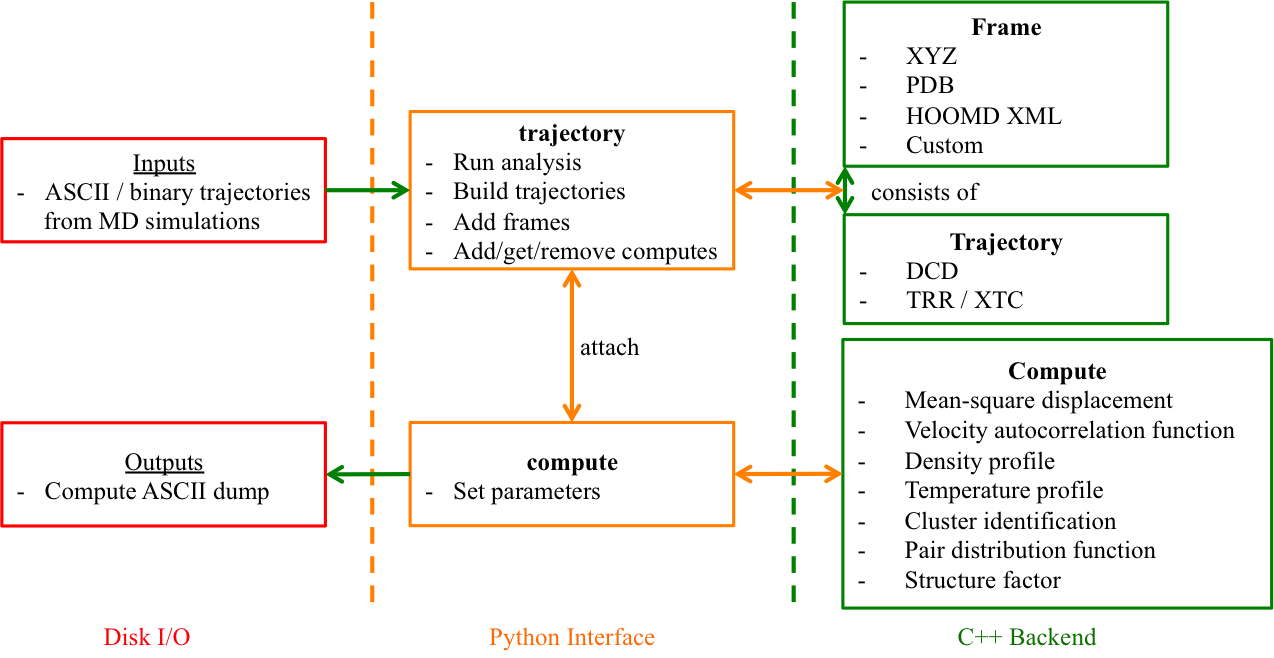
\includegraphics[width=0.8\textwidth]{layout}
 \caption{Diagram of software architecture. \label{fgr:arch}}
\end{figure}
\subsection{Basic organization}
The bulk of our code will be written in C++ with a Python wrapper interface (see diagram in Figure \ref{fgr:arch}). We choose to perform all calculations in C++ because in general reading frames and performing compute loops will be much faster in C++ than Python.

Our program will be organized around a central \verb=Trajectory= object. An array of \verb=Frame= objects is attached to \verb=Trajectory=. Each \verb=Frame= is a snapshot of the simulation at a certain time, and contains information about particle positions, velocities, types, masses, and diameters. We then attach \verb=Compute= objects to the \verb=Trajectory=. Each \verb=Compute= performs some type of analysis on the \verb=Trajectory=, such as calculating the average density profile, the mean-square displacement of atoms, etc. After initialization and attachment of all necessary \verb=Frame= and \verb=Compute= objects, the \verb=Trajectory= has a driving \verb=analyze()= method which (1) reads all \verb=Frame= objects into memory, and (2) calls all attached \verb=Compute= objects sequentially on the \verb=Trajectory=. Each \verb=Compute= dumps its output to disk as it finishes.

\subsection{User Interface}
For the typical user, all calculations will be interfaced through a Python module. The Python module will allow the user to:
\begin{enumerate}
\item{
Construct a \verb=Trajectory= via a simple initializer. For binary (complete) trajectories, the user need only specify the file name.
\begin{lstlisting}[language=python]
traj = trajectory.dcd(start_file='start.xml', binary_file='trajectory.dcd')
\end{lstlisting}
For frame-based trajectories, a simple Python wrapper for attaching frames will be included:
\begin{lstlisting}[language=python]
traj = trajectory.hoomd()
traj.addFrame(['dump.0.xml','dump.1.xml'])
traj.addFrame('dump.3.xml')
\end{lstlisting}
}
\item{Attach multiple \verb=Compute=s via a simple initializer.
\begin{lstlisting}[language=python]
traj = trajectory.dcd(...)
traj_2 = trajectory.hoomd(...)

my_compute = compute.msd(file_name='msd.dat', period=10.0)
traj.attach(my_compute)

my_other_compute = compute.density(file_name='density.dat', dx=0.1, dz=0.5)
traj_2.attach([my_compute,my_other_compute])
\end{lstlisting}
}
\item{Initialize trajectory analysis, which writes output to disk.
\begin{lstlisting}[language=python]
trajectory.analyze()
\end{lstlisting}
}
\end{enumerate} 
For the more advanced user, all important member variables and functions are exposed in the C++ classes directly. This provides a direct API for users to extend the current library with their own C++ code.

\subsection{External libraries}
We will capitalize on several existing external packages to simplify some tasks:
\begin{enumerate}
\item{\textbf{Boost} (\url{www.boost.org}).  We will use the Boost libraries for exporting to Python and to perform unit tests on the C++ code. Boost is a standard library on many high performance computing clusters, and also allows us to use smart pointers without requiring C++11 standards. Our code should then be backwards compatible for older operating systems and compilers, as is often the case for clusters maintained individually by groups rather than the university.}
\item{\textbf{pugixml} (\url{www.pugixml.org}). We will use the pugixml library to parse the HOOMD XML file format. pugixml is light-weight and only requires the compilation of a single file at runtime.}
\item{\textbf{NAMD DCD reader} (\url{http://www.ks.uiuc.edu/Research/namd/}). We will use the open sourced code from NAMD for reading DCD binary files. This is important because DCD files often have non-standard formatting.}
\end{enumerate}

\section{Scenarios}
\noindent\textbf{Scenario 1: Student or average researcher in molecular simulation field} \\
\noindent Molecular simulation programs generally have the capability to return information about the molecular trajectories to the user. The user performs structural and thermodynamic analysis on the results from the most popular molecular simulation packages, in-house, or legacy programs. The user easily analyzes the data from a simple Python script with built-in readers and computes.
   	 
\noindent\textbf{Scenario 2: Researcher using multiple simulation programs} \\
\noindent Users acquiring output from different simulation packages are often required to convert all files into a single format for post-processing. The user reads frames from multiple file types, and easily performs post-processing with only simple modifications in a single Python script.
   			 
\noindent\textbf{Scenario 3: Researcher performing advanced analysis} \\
\noindent The user may access the C++ API to extend the current code base, either as a plugin for the user for a specific application or as a contribution to the main code base for more broadly useful routines. For example, if the user wishes to calculate Maxwell-Stefan transport coefficients for mixtures they can extend the mean-squared displacement and/or velocity autocorrelation compute(s).

\section{Milestones}
\subsection*{Prototype (5 Dec 2014)}
\begin{itemize}
\item{\textbf{Base classes / C++ API.} Base classes for \verb=Trajectory=, \verb=Frame=, and \verb=Compute=, to be extended for specific implementations. Headed by Mike Howard.}
\item{\textbf{Export to Python}. Boost Python module export of C++ classes. Allows for quick testing of interface. Headed by Sang Beom Kim and Elia Altabet.}
\item{\textbf{HOOMD XML.} Representative implementation of a \verb=Frame=. Necessary to test \verb=Compute= on real data. Headed by Andrew Santos.}
\item{\textbf{Density profile compute.} Representative implementation of a \verb=Compute=. Needed to validate \verb=Trajectory.analyze()= loop is functional. Headed by Joey Vella.}
\end{itemize}

\subsection*{Alpha version (12 Dec 2014)}
\begin{itemize}
\item{\textbf{Additional readers completed.} XYZ file format and PDB file format. Allows for testing of trajectories compiled from different frames. Headed by Joey Vella and Sang Beom Kim.}
\item{\textbf{Additional computes completed.} Mean-square displacement and pair distribution function. Headed by Andrew Santos and Elia Altabet.}
\item{\textbf{Python module written.} Python classes and helper functions for user interface to wrap C++ methods. Headed by Mike Howard.}
\end{itemize}

\subsection*{Beta version (6 Jan 2015)}
\begin{itemize}
\item{\textbf{Fully implement proposed reader formats.} Includes additional ASCII and binary file formats. Headed by Andrew Santos and Sang Beom Kim.}
\item{\textbf{Fully implement proposed computes.} Headed by Joey Vella and Elia Altabet.}
\item{\textbf{Finalize Python interface.} Complete Python module for all additional classes, and refine user interface. Headed by Mike Howard.}
\end{itemize}

\section{Future Features}
We considered additional features for our project that we believe to currently be beyond the scope of what can be accomplished. However, we will look to incorporate these features into our software in the future for use in our research groups. Planned future features include:
\begin{itemize}
\item{\textbf{Interconversion of file formats.} (target v. 0.1). Given that trajectories are currently read into memory as a simple structure, we can add the ability to now \emph{export} this data to allow for convenient interconversion. This may be especially useful if parsing an ASCII format into a binary format.}
\item{\textbf{Topologies.} (target v. 0.2). The initial version of our project will not consider the calculation of properties that rely on knowledge of the bond structure (topology) of the system being studied.  Additional computes could be added for topology-dependent properties.  For example if one is interested in gyration tensor of a system of polymers, information on how monomers are bonded would be required.  This would also require the augmentation of readers in order to read in topology information.}
\item{\textbf{OpenMPI.} (target v. 0.3). Many of the computed properties of trajectories have algorithms that are trivially parallelizable, and so a parallel implementation of the C++ code presents an opportunity for considerable computational speed-up. Parallelization across multiple nodes has the potential to significantly reduce memory requirements because the entire trajectory may not be needed for each parallel rank. An OpenMPI implementation of our code is then an attractive option for performing calculations on large trajectories where computational time and memory are limiting.}
\end{itemize}

\end{document}